\chapter{実験}
\section{シミュレーション}
シュミレーションを利用して,設計した制御系の性能を確認する.

\subsubsection{シミュレーションソフト}
シミュレーションには数値計算ソフト「Scilab」に付属しているビジュアルモデリングソフト「Xcos」を使用する.Xcosで組み立てたブロック線図を図\ref{fig:blockXcos}に示す.この際、リフトにかかる電圧の絶対値の最大は実際と同じく12[v]に制限した.

\begin{figure}[htbp]
  \begin{center}
    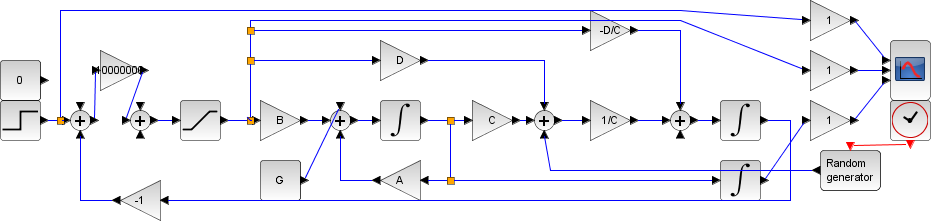
\includegraphics[width=150mm]{img/blockXcos.png}
    \end{center}
  \caption{Xcosで組み立てたブロック線図}
 \label{fig:blockXcos}
\end{figure}

\subsubsection{シミュレーション結果}
シミュレーションの結果を図\ref{fig:sim}に示す.

\begin{figure}[htbp]
 \begin{center}
    \includegraphics[width=150mm]{img/sim.bmp}
    \end{center}
  \caption{入力した目標値による電圧と位置の時間変化}
 \label{fig:sim}
\end{figure}

\subsubsection{測定誤差の影響}
実際に電流を測定した時には誤差があると考え,誤差の影響を見るため電流の値を分散が1[A]の正規分布になるようにした.その際のシミュレーション結果を図\ref{fig:sim}に示す.

\begin{figure}[htbp]
 \begin{center}
    \includegraphics[width=150mm]{img/sim2.bmp}
    \end{center}
  \caption{入力した目標値による電圧と位置の時間変化}
 \label{fig:sim}
\end{figure}

電圧のグラフが激しく振動している為,塗りつぶされて見える.これは電流のノイズの影響だと考えられるが,ノイズの平均値が0ならば現在位置に影響はなかった.

\section{検出誤差の確認}
電流センサが検出する電流と実際に流れている電流に誤差があると,リフトの速度推定にも誤差が生じてしまい,時間がたつにつれリフトの位置がずれていってしまう.ここでは電流センサで検出した値がどれだけの測定誤差を持つのか確認する.

\subsubsection{使用機器}
モータドライバは電流センサを内蔵したものを使用した.使用したモータドライバを図\ref{fig:currentDriver}に示す.使用した機器一覧を表\ref{tab:partsCurrent}に示す.

\begin{figure}[htbp]
 \begin{center}
    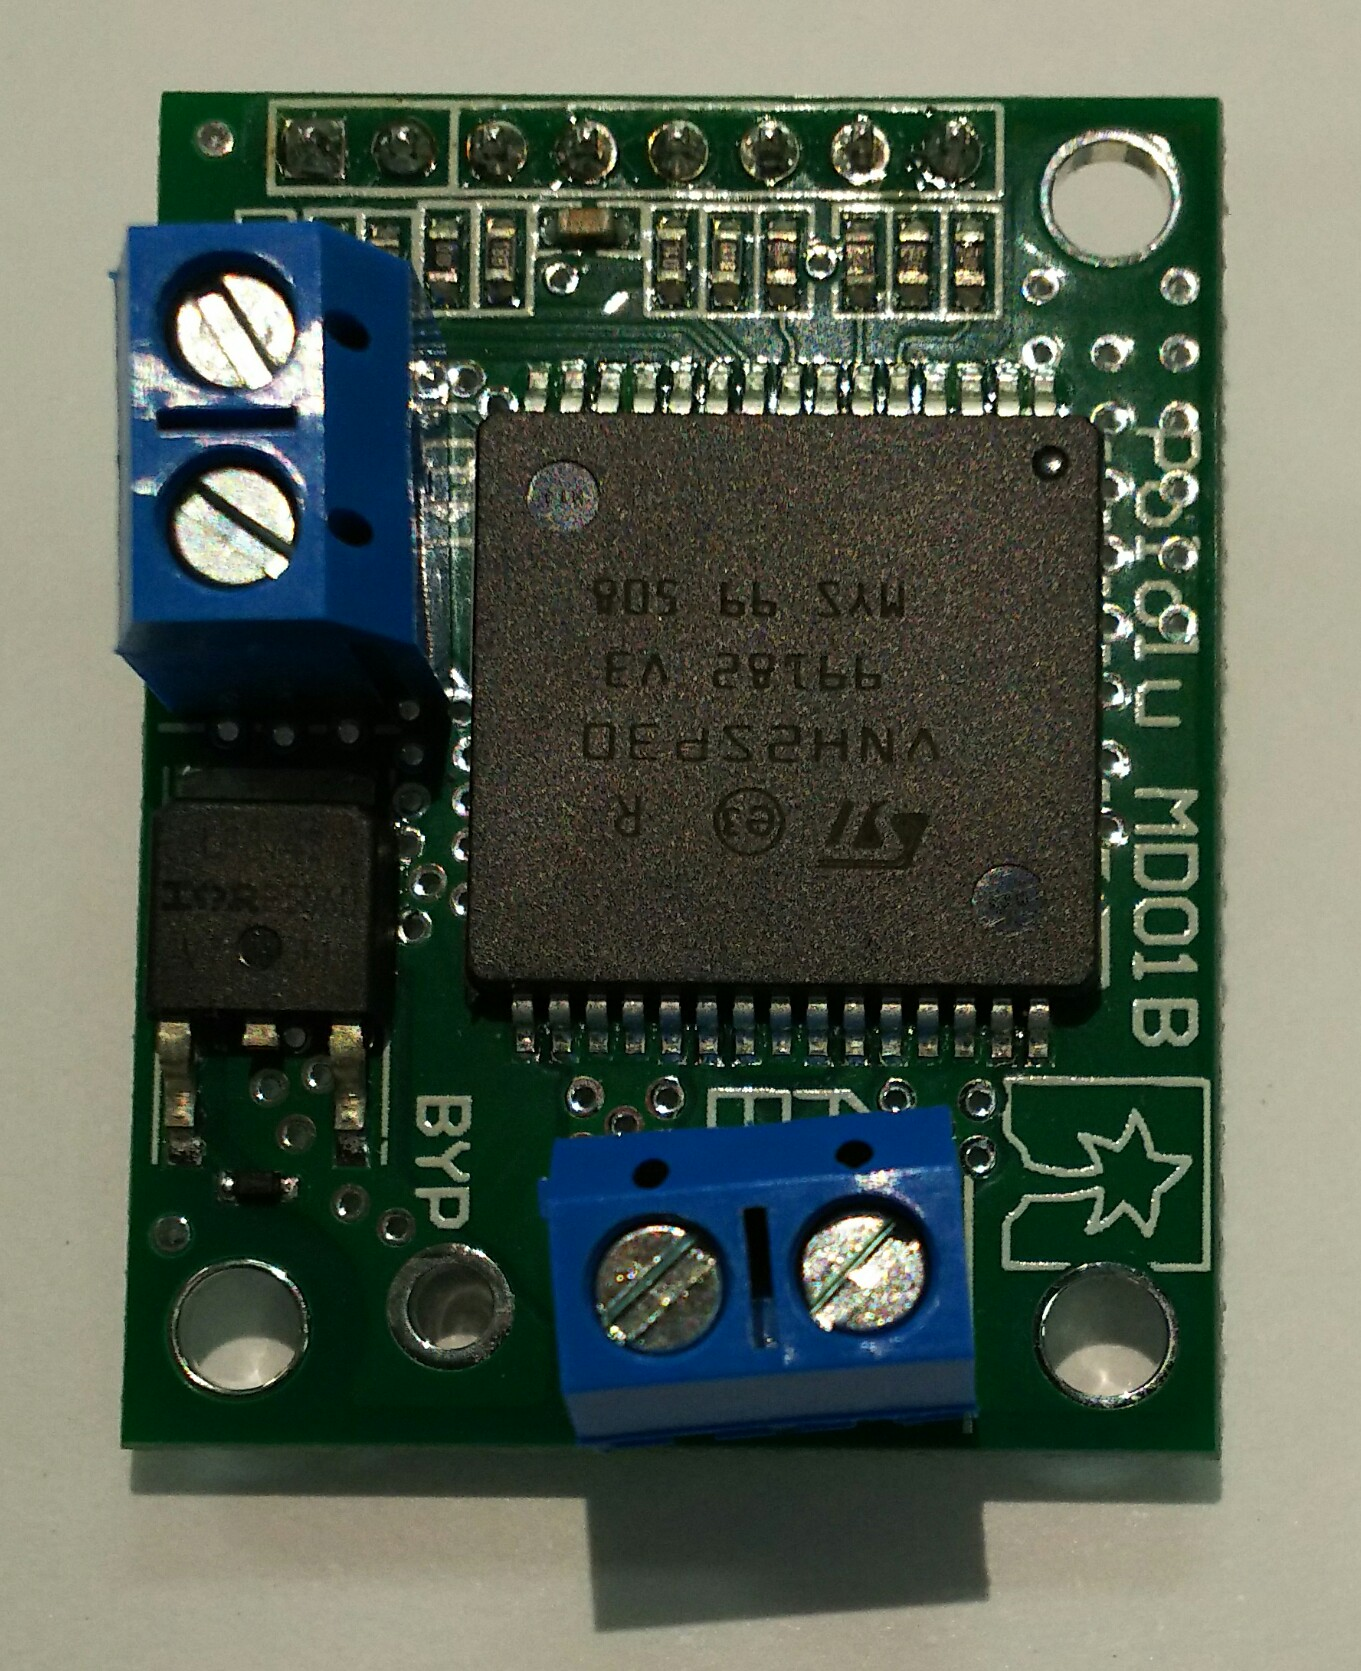
\includegraphics[width=75mm]{img/currentDriver.JPG}
    \end{center}
  \caption{電流センサ内臓モータドライバ}
 \label{fig:currentDriver}
\end{figure}

\begin{table}[htb]
 \begin{center}
  \caption{搭載部品の型番とメーカ}
  \begin{tabular}[htbp]{|c|c|c|}
   \hline
   製品名&型番&メーカ \\
   \hline
   arduino&ArduinoUno&Arduino SRL\\
   \hline
   DCモータ&組み合わせモータ323726&マクソン\\
   \hline
   電流センサ内臓モータドライバ&MD01B&Pololu\\
   \hline
   テスター&VOAC86&IWATU\\
   \hline
  \end{tabular}
  \label{tab:partsCurrent}
 \end{center}
\end{table}

\subsubsection{計測方法}
モータに電圧を12[v]印加し.電流センサから値を1ミリ秒ごとに記録し,平均とノイズの分散を算出する.その後,テスターで実際の電流を計測し,電流センサで得た平均値との差をノイズの平均値とする.

\subsubsection{電流計測}
電流を計測した結果を図\ref{fig:currentMeasurement}に示す.

\begin{figure}[htbp]
 \begin{center}
    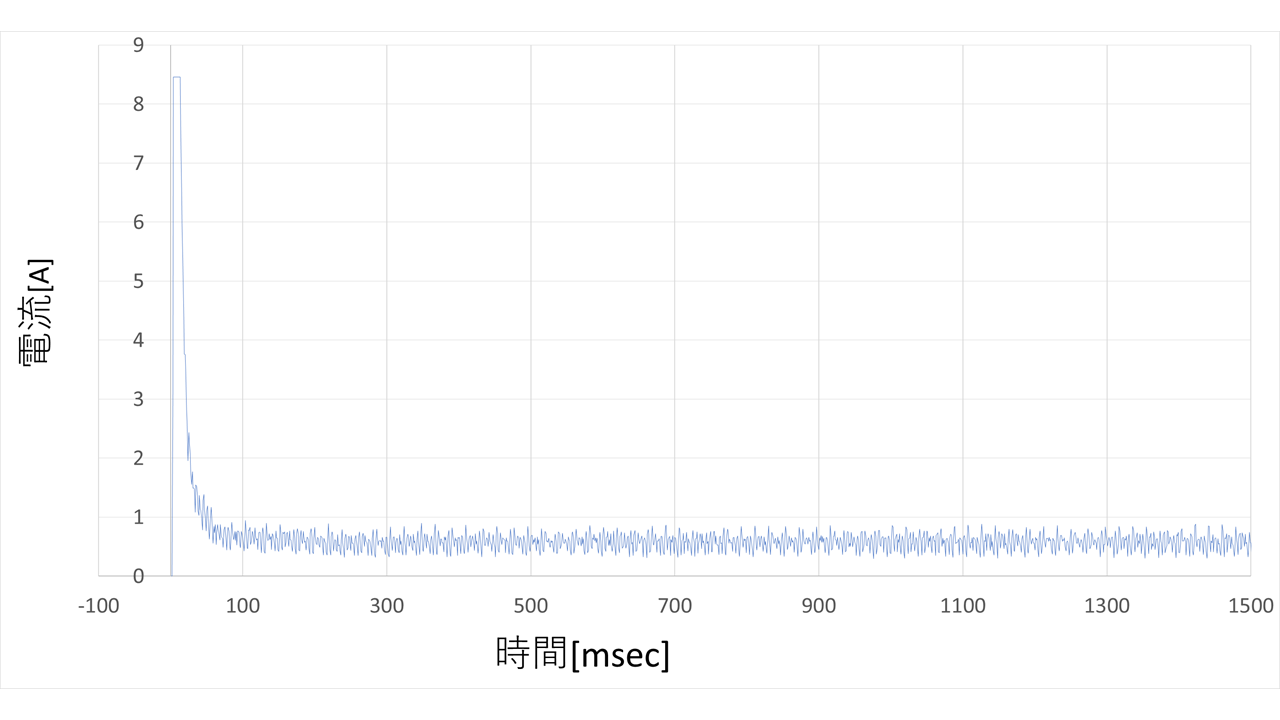
\includegraphics[width=150mm]{img/currentMeasurement.png}
    \end{center}
  \caption{電流の時間変化}
 \label{fig:currentMeasurement}
\end{figure}

平均は0.575[A],ノイズの分散は1.880[A],テスターでの計測結果は0.232[A]となった.よってノイズの平均は0.343[A]となった.
